\section{Desáté cvičení}
 
\section*{Algoritmus CYK}

\subsection{Příklad} % 10.1 

Je dána gramatika $\mathcal{G} = (N, \Sigma, S, P)$, kde 
$N = \{S, A, B, C, D\}$, $\Sigma = \{a, b\}$ a pravidla $P$ jsou dána:
\vspace*{-4mm}
\[
    \begin{array}{l l}
        P: & S \rightarrow AB \mid CS \mid AD \\
           & A \rightarrow AC \mid AD \mid a \\
           & B \rightarrow BC \mid b \\
           & C \rightarrow DS \mid SC \mid a \\
           & D \rightarrow BA \mid b \\
    \end{array}
\]

Algoritmem CYK rozhodněte, zda gramatika $\mathcal{G}$ generuje slova $w_1$ a $w_2$, kde $w_1 = aaaba$ a $w_2 = abbaa$.  
Pokud ano, nakreslete derivační strom a napište jemu odpovídající levou derivaci.
\vspace*{3mm}

slovo $w_1$:

\begin{minipage}{0.5\textwidth}
\[
\hspace*{-20mm}
\begin{array}{r c l}

    AB & \leftarrow &S \\
    AC & \leftarrow &A \\
    AD & \leftarrow &S, A \\
    BA & \leftarrow &D \\
    BC & \leftarrow &B \\
    CS & \leftarrow &S \\
    DS & \leftarrow &C \\
    SC & \leftarrow &C \\
\end{array}
\]


\begin{NiceTabular}{ccccc}[hvlines, corners = NE] % NE = north east
    $C,A, S$ &   &   &   &   \\ 
    $S, A$ & $C, A, S$ &   &   &   \\ 
    $A$ & $S,A$ & $S,A, C$ &   &   \\ 
    $A$ & $A$ & $S,A$ & $D,B$ &   \\ 
    $A,C$ & $A, C$ & $A,C$ & $B,D$ & $A,C$ \\ 
    $a$ & $a$ & $a$ & $b$ & $a$ \\ 
\end{NiceTabular}


\end{minipage}\begin{minipage}{0.5\textwidth}
    

    \begin{center}
        
        \begin{forest}
            for tree={
                grow=south,                 % Tree grows downward
                edge={->},                  % Draw edges as arrows
                align=center,               % Center the text inside nodes
            }
            [$S$
                [$C$
                    [$a$]
                ]
                [$S$
                    [$C$
                        [$a$]
                    ]
                    [$S$
                        [$A$
                            [$a$]
                        ]
                        [$D$
                            [$B$
                                [$b$]
                            ]
                            [$A$
                                [$a$]
                            ]
                        ]
                    ]
                ]
            ]
        \end{forest}    \end{center}
    

\end{minipage}

$$S \stackrel{S \rightarrow CS}{\Longrightarrow} CS \stackrel{C \rightarrow a}{\Longrightarrow} aS \stackrel{S 
\rightarrow CS}{\Longrightarrow} aCS \stackrel{C \rightarrow a}{\Longrightarrow} aaS \stackrel{S \rightarrow AD}
{\Longrightarrow} aaAD \stackrel{A \rightarrow a}{\Longrightarrow} aaaD \stackrel{D \rightarrow BA}{\Longrightarrow} 
aaaBA \stackrel{B \rightarrow b}{\Longrightarrow} aaabA \stackrel{A \rightarrow a}{\Longrightarrow} aaaba$$

\vspace*{-2mm}
slovo $w_2$: \\
\begin{minipage}{0.5\textwidth}
    
\begin{NiceTabular}{ccccc}[hvlines, corners = NE] % NE = north east
    $C,A, S$ &   &   &   &   \\ 
    $C, A, S$ & $ - $ &   &   &   \\ 
    $S,A$ & $- $ & $D,B$ &   &   \\ 
    $S,A$ & $- $ & $D,B$ & $A$ &   \\ 
    $A,C$ & $B,D$ & $B,D$ & $A,C$ & $A,C$ \\ 
    $a$ & $b$ & $b$ & $a$ & $a$ \\ 
\end{NiceTabular}

\end{minipage}
\begin{minipage}{0.5\textwidth}
    

\begin{center}
        
    \begin{forest}
        for tree={
            grow=south,                 % Tree grows downward
            edge={->},                  % Draw edges as arrows
            align=center,               % Center the text inside nodes
        }
        [$S$
            [$A$
                [$A$
                    [$a$]
                ]
                [$D$
                    [$b$]
                ]
            ]
            [$D$
                [$B$
                    [$b$]
                ]
                [$A$
                    [$A$
                        [$a$]
                    ]
                    [$C$
                        [$a$]
                    ]
                ]
            ]
        ]
    \end{forest}    \end{center}

\end{minipage}
\vspace*{-5mm}
$$S \stackrel{S \rightarrow AD}{\Longrightarrow} AD \stackrel{A \rightarrow AD}{\Longrightarrow} ADD \stackrel{A 
\rightarrow a}{\Longrightarrow} aDD \stackrel{D \rightarrow b}{\Longrightarrow} abD \stackrel{D \rightarrow BA}
{\Longrightarrow} abBA \stackrel{B \rightarrow b}{\Longrightarrow} abbA \stackrel{A \rightarrow AC}{\Longrightarrow} 
abbAC \stackrel{A \rightarrow a}{\Longrightarrow} abbaC \stackrel{C \rightarrow a}{\Longrightarrow} abbaa$$

% \includegraphics[width=1\textwidth]{CYK.jpg}

\subsection{Příklad} % 10.2

Je dána gramatika $\mathcal{G} = (N, \Sigma, S, P)$, kde 
$N = \{S, A, B, C, D\}$, $\Sigma = \{a, b\}$ a pravidla $P$ jsou dána:\[
    \begin{array}{l l}
        P: & S \rightarrow AB \mid AC \mid BC \\
           & A \rightarrow AD \mid a \\
           & B \rightarrow BD \mid b \\
           & C \rightarrow AB \mid BB \\
           & D \rightarrow a \mid b \\
    \end{array}
\]

Algoritmem CYK rozhodněte, zda slovo $w_1 = abaab$ je touto gramatikou generováno. Pokud ano, nakreslete derivační strom 
a napište levou derivaci.

$w_1 = abaab$: 

\begin{minipage}{0.5\textwidth}
    

\begin{NiceTabular}{ccccc}[hvlines, corners=NE]
    D, C, B, S &   &   &   &   \\
    D, C, A, S & S, D, C, B &   &   &   \\
    A, S, C & C & D, B, C &   &   \\
    D, C & S, A & C, S & D, C &   \\
    A, D & B, C & A, D & A, D & B, C \\
    a & b & a & a & b \\
\end{NiceTabular}
\end{minipage}
\begin{minipage}{0.5\textwidth}
    

\begin{center}
    \begin{forest}
        for tree={
            grow=south,                 % Tree grows downward
            edge={->},                  % Draw edges as arrows
            align=center,               % Center the text inside nodes
        }
        [$S$
            [$C$
                [$D$
                    [$a$]
                ]
                [$C$
                    [$a$]
                ]
            ]
            [$D$
                [$C$
                    [$A$
                        [$a$]
                    ]
                    [$A$
                        [$a$]
                    ]
                ]
                [$B$
                    [$b$]
                ]
            ]
        ]
    \end{forest}
    \end{center}
\end{minipage}

$S \stackrel{S \rightarrow CD}{\Longrightarrow} CD \stackrel{C \rightarrow DC}{\Longrightarrow} DCD \stackrel
{D \rightarrow a}{\Longrightarrow} aCD \stackrel{C \rightarrow b}{\Longrightarrow} abD \stackrel{D \rightarrow CB}
{\Longrightarrow} abCB \stackrel{C \rightarrow AA}{\Longrightarrow} abAAB \stackrel{A \rightarrow a}{\Longrightarrow} 
abaAB \Longrightarrow $\\
$\stackrel{A \rightarrow a}{\Longrightarrow} abaaB \stackrel{B \rightarrow b}{\Longrightarrow} abaab$

\subsection{Příklad - NEBUDE U ZKOUŠKOVÝHO TESTU !!}

S využitím Pumping Lemmatu ukažte, že následující jazyk není bezkontextový, kde $$L = \{ww; w \in\{a,b\}^{\star}\}$$


\textbf{Pumping Lemma.} Pro každý CF jazyk $L$ existuje přirozené číslo $m \geq 1$ takové, že každé slovo $z \in L$ 
délky alespoň $m$ lze rozdělit na pět částí $z = uvwxy$ tak, že:

\begin{itemize}[label=\textbullet]
    \item $\lvert vwx \rvert \leq m$, (tj. prostřední část není příliš dlouhá),
    \item $vx \neq \varepsilon$ (tj. alespoň jedno ze slov $v$, $x$ není prázdné),
    \item pro všechna $i \geq 0$ platí $uv^i wx^i y \in L$, (tj. $v$ a $x$ se dají do slova „napumpovat“ a stále 
    dostaneme slovo z jazyka $L$).
\end{itemize}

spoiler alert: nedoděláno 

Zvolíme $z = a^m b^m a^m b^m \, \in L$, $|z| = 4m > m$. \\ 
$\dots$\\
$\dots$\\
$\dots$\\

Máme 7 možností: 
% \begin{center}
%     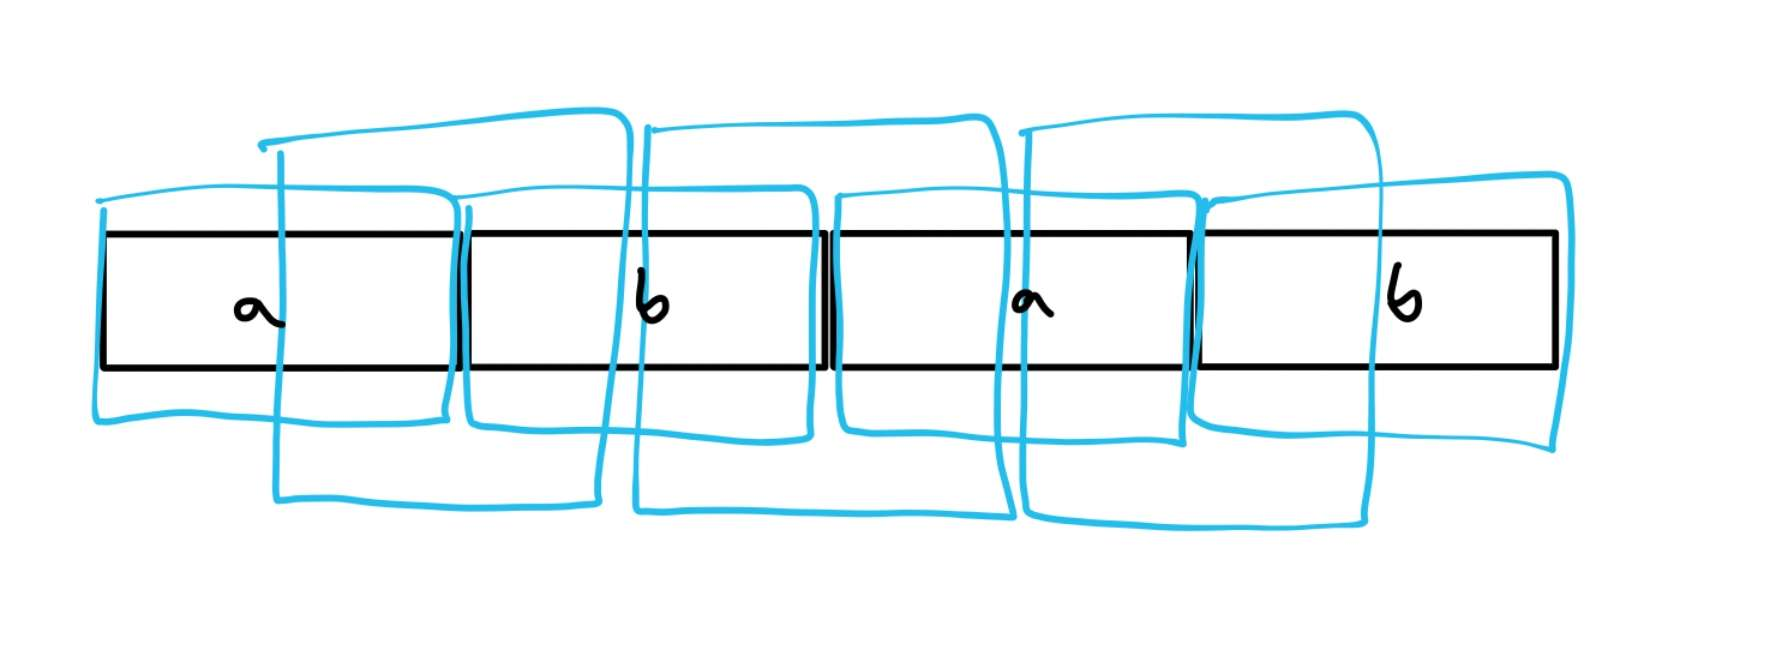
\includegraphics[width=0.3\textwidth]{7moznosti.jpg}
% \end{center}
Takže to dělat nebudeme. 

% pumping lemma intuice: 
% \begin{center}
%     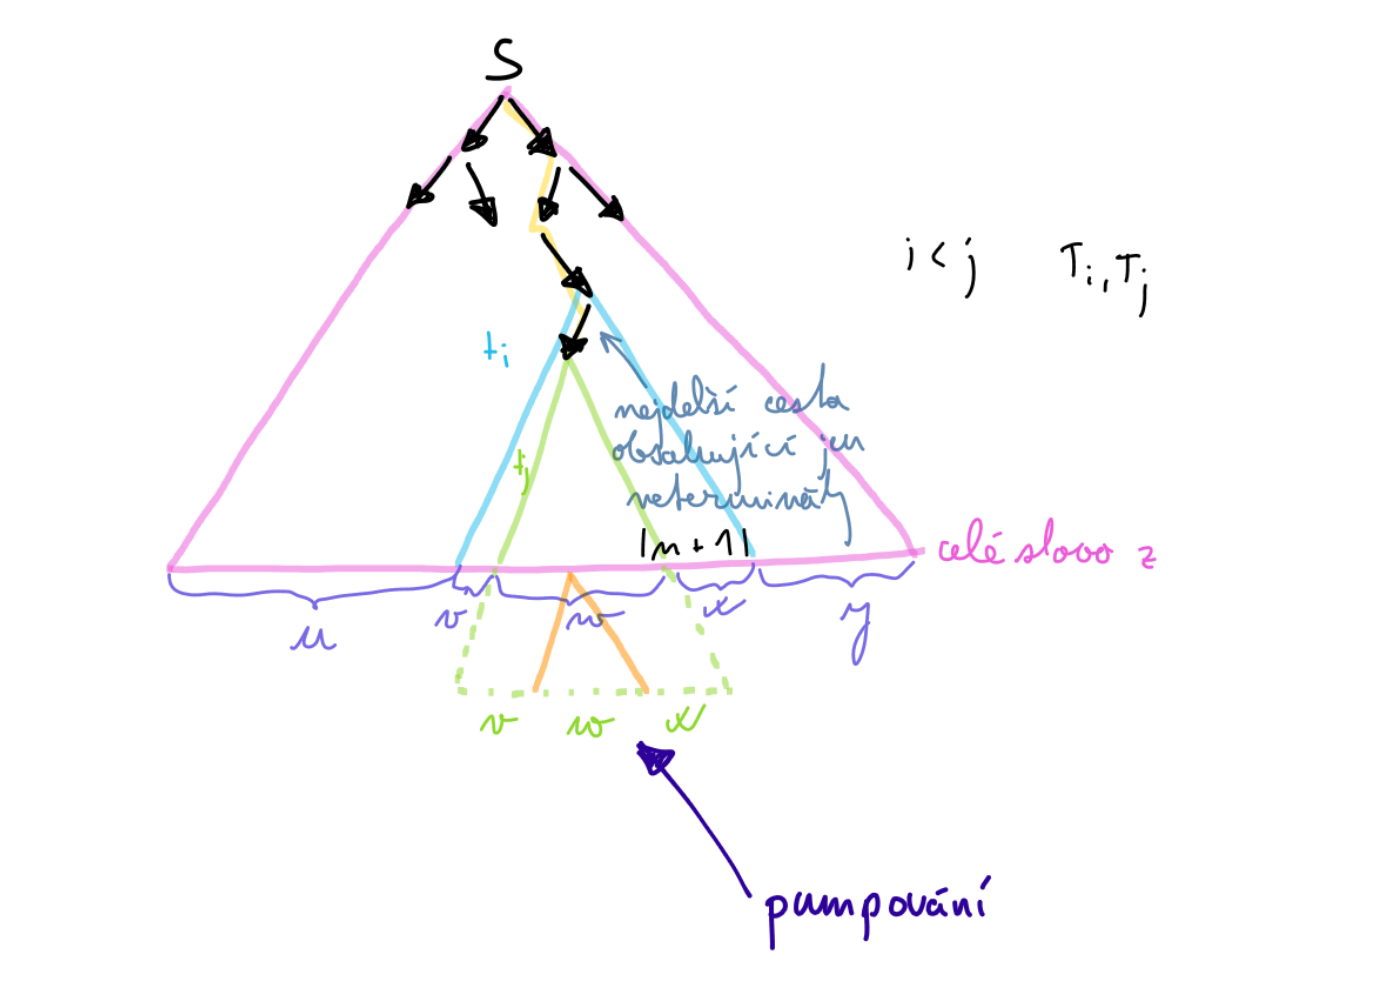
\includegraphics[width=0.5\textwidth]{pl_intuice.png}
% \end{center}

\subsection{Příklad} % 10.4 
Je dána CF gramatika $\mathcal{G} = (N, \Sigma, S, P)$, kde $N = \{S, A, B, C\}$, $\Sigma = \{a, b\}$ a $P$ je:

\[
\begin{array}{l l}
    P: & S \rightarrow SA \mid aSb \mid Cb \\
       & A \rightarrow SC \mid \varepsilon \\
       & B \rightarrow bAB \mid bS \mid AA \\
       & C \rightarrow CB \mid bA \mid a \\
\end{array}
\]

Pomocí matematické indukce dokažte, že:
\[
A \Rightarrow_{\G}^{\star} S^i A C^i
\]
pro všechna $i \geq 0$. Toho využijte k důkazu, že $(ab)^{i+1}(ab^3)^i$ jsou generována gramatikou $\mathcal{G}$ pro 
každé $i \geq 0$.

1) Základní krok: $i = 0$

Pro $i = 0$, platí:
\[
A \stackrel{A \rightarrow \varepsilon}{\Longrightarrow} A
\]
což odpovídá:
\[
S^0 A C^0 = A \quad \checkmark
\]

2) Indukční krok:

předp. $A \implies^{\star} S^n a C^n$, chceme dokázat $A \implies^{\star} S^{n+1} A C^{n+1}$.

$A \stackrel{A \rightarrow SC}{\Longrightarrow} SC \stackrel{S \rightarrow SA}{\Longrightarrow} SAC \stackrel{I.P.}
{\Longrightarrow}^{\star} SS^nAC^nC$

nebo

$A \stackrel{I.P.}{\Longrightarrow} S^n A C^n \stackrel{A \rightarrow SC}{\Longrightarrow} S^nSCC^n \stackrel
{S \rightarrow SA}{\Longrightarrow} S^nSACC^n$.



\subsection{Příklad} % 10.5 
Je dána gramatika $\mathcal{G} = (N, \Sigma, S, P )$, kde $N = \{S, A, B, C, D\}$, $\Sigma = \{a, b, c\}$ a
pravidla~$P$ jsou dána
\[
% \hspace*{-85mm}
\begin{array}{l l}
    P: & S \rightarrow AB \mid CD \mid AC\\
    & A \rightarrow AC \mid a \\
    & B \rightarrow BD \mid b \\
    & C \rightarrow AD \mid a \\
    & D \rightarrow BA \mid b \\ 
\end{array}
\]

Algoritmem CYK rozhodněte, zda gramatika $\mathcal{G}$ generuje slova $w_1$ a $w_2$, kde $w_1 = baaba$ a $w_2 = abaaa$.
 Pokud ano, nakreslete derivační strom a napište jemu odpovídající levou derivaci.


\begin{minipage}{0.5\textwidth}
    

\[
    \begin{array}{l l}
    & AB \leftarrow S \\
    & AC \leftarrow S, A \\
    & AD \leftarrow C \\
    & BA \leftarrow D \\
    & BD \leftarrow B \\ 
    & CD \leftarrow S \\ 
    \end{array}
\]
\end{minipage}\begin{minipage}{0.5\textwidth}
    
slovo $w_1 = baaba$: 

\vspace*{2mm}

\begin{NiceTabular}{ccccc}[hvlines, corners = NE] % NE = north east
    $D$ &  &   &   &   \\ 
    $D$ & $S, A, C$ &  &   &   \\ 
    $D$ & $S, C, A$ & $C, S$ &  &  \\ 
    $D$ & $S, A$ & $S, C$ & $D$ &  \\ 
    $B, D$ & $A,C$ & $A,C$ & $B, D$ & $A, C$ \\ 
\end{NiceTabular}

\hspace*{5mm}$b$ \hspace*{10mm} $a$ \hspace*{10mm} $a$ \hspace*{9mm} $b$ \hspace*{8mm} $a$
    
\vspace*{2mm}
    Gramatika $\mathcal{G}$ negeneruje slovo $w_1$. 

\end{minipage}


\begin{minipage}{0.5\textwidth}
    slovo $w_2 = abaaa$: 
    
    \begin{NiceTabular}{ccccc}[hvlines, corners = NE] % NE = north east
        $C,S$ &   &   &   &   \\ 
        $C, S$ & $D$ &   &   &   \\ 
        $C,S$ & $D$ & $S,A$ &   &   \\ 
        $S,C$ & $D$ & $S,A$ & $S,A$ &   \\ 
        $A,C$ & $B, D$ & $A,C$ & $A,C$ & $A,C$ \\ 
    \end{NiceTabular}
    
\hspace*{5mm}$a$ \hspace*{8mm} $b$ \hspace*{8mm} $a$ \hspace*{8mm} $a$ \hspace*{8mm} $a$


        \vspace*{2mm}
        Gramatika $\mathcal{G}$ generuje slovo $w_2$. 
        
        \vspace*{3mm}

        Levá derivace: 

            \begin{align*}
                        & S\stackrel{S \rightarrow CD}{\Longrightarrow} CD 
                        \stackrel{C \rightarrow a}{\Longrightarrow} aD 
                        \stackrel{D \rightarrow BA}{\Longrightarrow} aBA  
                        \stackrel{B \rightarrow b}{\Longrightarrow} abA \Longrightarrow\\
                        &\stackrel{A \rightarrow AC}{\Longrightarrow} abAC 
                    \stackrel{A \rightarrow AC}{\Longrightarrow} abACC 
                    \stackrel{A \rightarrow a}{\Longrightarrow} abaCC \Longrightarrow\\
                  &\stackrel{C \rightarrow a}{\Longrightarrow} abaaC 
                    \stackrel{C \rightarrow a}{\Longrightarrow} abaaa
            \end{align*}
        
\end{minipage}\begin{minipage}{0.5\textwidth}
    

    Derivační strom pro slovo $w_2$:
    \vspace*{5mm}
    \begin{center}
        
        \begin{forest}
            for tree={
                grow=south,                 % Tree grows to the right
                edge={->},                  % Draw edges as arrows
                % draw,                       % Draw the nodes
                % rounded corners,           % Rounded corners for nodes
                align=center,                % Center the text inside nodes, 
                }
                [$S$
                    [$C$
                        [$a$]
                    ]
                    [$D$
                        [$B$
                            [$b$]
                        ]
                        [$A$
                            [$A$
                                [$A$
                                    [$a$]
                                ]
                                [$C$
                                    [$a$]
                                ]
                            ]
                            [$C$
                                [$a$]
                            ]
                        ]
                    ]
                ]
            \end{forest}
        \end{center}
\end{minipage}